\section{Przegląd dostępnych rozwiązań dostępnych na rynku}
\label{sec:solutions}



\subsection{Hadoop}
\label{sec:solutions:hadoop}



\subsection{Hive}
\label{sec:solutions:hive}



\subsection{Spark (Stream Spark)}
\label{sec:solutions:spark}

Apache Spark to projekt, którego częścią jest Apache Spark Streaming, czyli framework, który umożliwia przetwarzanie strumieniowych, stale napływających o dużej częstotliwości danych w czasie rzeczywistym. Dane mogą pochodzić z różnych źródeł, takich jak Kafka, Flume, ZeroMQ, czy natywne gniazda TCP (czyli implementacja zaproponowana w \ref{sec:eventgenerator-eventreceiver}). Przetworzone dane mogą być składowane na dysku, w bazach danych, wysyłane na szyny danych. Spark dostarcza również wbudowane algorytmy uczenia maszynowego (ang. \emph{machine learning}) oraz analizowania grafów (ang. \emph{graph processing}). Dane są definiowane pojęciem RDD\cite{manual-apache-spark-streaming} i nie zmieniają swojego stanu (\emph{immutable state}).

\begin{figure}[h!]
  \centering
    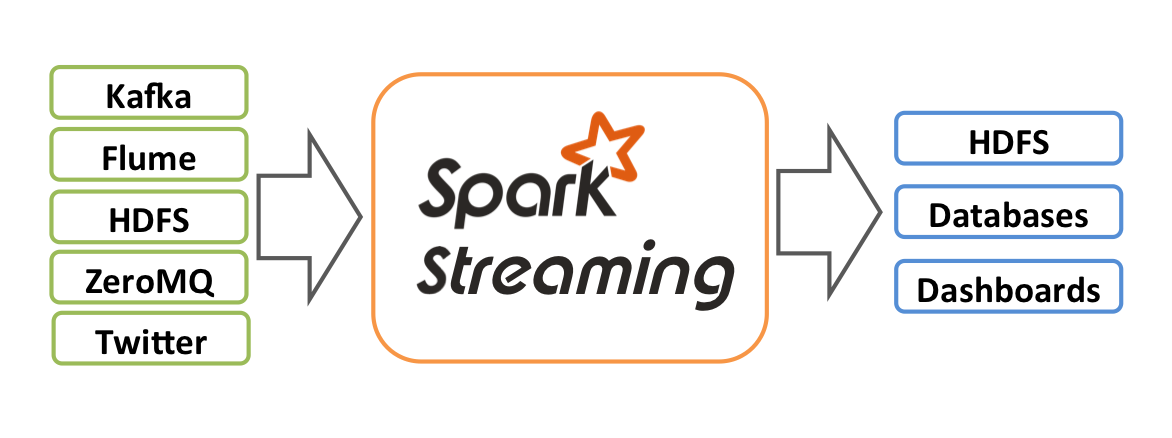
\includegraphics[scale=0.75]{spark-streaming-arch.png}
  \caption{Zasada działania Apache Spark Stream}
  \label{fig:spark-streaming-arch}
\end{figure}

Apache Spark Streaming umożliwia również obliczenia na przesuwnym oknie RDD:

\begin{figure}[h!]
  \centering
    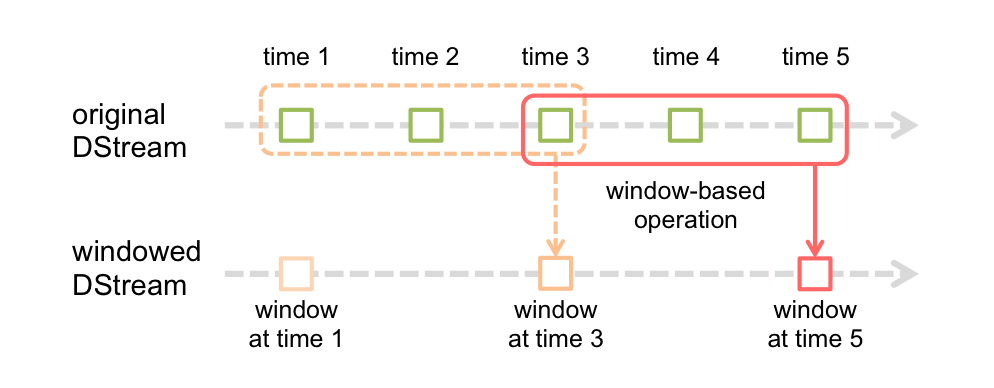
\includegraphics[scale=0.75]{spark-streaming-dstream-window.png}
  \caption{Przesuwne okno czasowe w Apache Spark Streaming}
  \label{fig:spark-streaming-dstream-window}
\end{figure}

Wykorzystanie Spark Streaming umożliwia wykonywanie operacji na strumieniu danych znanych z MapReduce oraz strumieniowych baz danych, w szczególności:

\begin{itemize}[noitemsep]
  \item map
  \item reduce
  \item filter
  \item transform
  \item union - złączenie źródeł danych
  \item count oraz countByValue
\end{itemize}
